\documentclass[11pt]{article}
\usepackage[utf8]{inputenc}
\usepackage[margin=3.cm]{geometry}
\usepackage{cite}
\usepackage{graphicx}
\usepackage{amsthm}
\usepackage{amsmath}
\usepackage{amsfonts}
\usepackage{amssymb}
\usepackage{enumerate} % for specifying (a), i., IV, etc 
\usepackage{mathrsfs} % for \mathscr D for distributions
\usepackage{mathtools} % :=f
\usepackage[colorlinks]{hyperref} % color 
\usepackage{multirow} % multirow
\usepackage[toc,page]{appendix} %appendix
\usepackage{algorithm} % algorithmt
\usepackage[noend]{algpseudocode}
\usepackage{bbm} % indicator function
%\usepackage[square]{natbib} % citation 
\usepackage[square]{natbib} % citation 
\hypersetup{colorlinks,linkcolor={blue},citecolor={blue},urlcolor={red}}  
\usepackage{array}     % and/or
\usepackage{longtable} % and/or
\usepackage{hyperref} %link
\usepackage{wrapfig}
\usepackage{multirow}



\usepackage[flushleft]{threeparttable} % table notes

% AA: I commented the follwoing package since it was using pstricks which I don't have installed
%\usepackage{colortab}  % or  
\usepackage{colortbl}
\usepackage{arydshln} % dashed line

%\usepackage{tikz}
% \usetikzlibrary{arrows.meta}
\usepackage{blkarray, bigstrut}
\usepackage{xparse}

\usepackage{setspace}
\onehalfspace

\theoremstyle{remark}

\usepackage{pgfplots}
\usetikzlibrary{arrows.meta}

\newcommand\Lc{\mathscr L}
\newcommand\lchol{\Lc_{\text{chol}}}
\newcommand\Sigh{\widehat \Sigma}

%%%%

\newcommand{\f}{\frac}
\newcommand{\p}{\partial}

% Number systems %
\newcommand{\Z}{\mathbb{Z}}
\newcommand{\N}{\mathbb{N}}
\newcommand{\Q}{\mathbb{Q}}
\newcommand{\R}{\mathbb{R}}
%\newcommand{\C}{\mathbb{C}}
\newcommand{\F}{\mathbb{F}}
\newcommand{\BH}{\matbb{H}}
\newcommand{\BP}{\mathbb{P}}
\newcommand{\B}{\calB}
\newcommand{\E}{\mathbb{E}}
\newcommand{\T}{\mathbb{T}}

\let\temp\P
\let\P\BP
%% Probability %%
\newcommand\independent{\protect\mathpalette{\protect\independenT}{\perp}}
\def\independenT#1#2{\mathrel{\rlap{$#1#2$}\mkern2mu{#1#2}}}

% % Analysis shortcuts % %
\newcommand{\eps}{\varepsilon}
\newcommand{\el}[1]{\ell^{#1}(\mathbb{N})} % little l^p spaces
\newcommand{\elinf}{\ell^{\infty}(\mathbb{N})}
\newcommand{\pnorm}[2]{\left\|#1\right\|_{#2}}
\newcommand{\norm}[1]{\left\|#1\right\|}
\newcommand{\ip}[2]{\left\langle #1, #2 \right\rangle}
\newcommand{\ceil}[1]{\lceil #1 \rceil}
\newcommand{\floor}[1]{\lfloor #1 \rfloor}
\newcommand{\dd}[2]{\frac{\mathrm{d} #1}{\mathrm{d} #2}}
\newcommand{\ddyddx}[2]{\frac{\mathrm{d}^2 #1}{\mathrm{d} {#2}^2}}
\newcommand{\ddx}[1]{\frac{\mathrm{d}}{\mathrm{d} #1}}
\newcommand{\ddddx}[1]{\frac{\mathrm{d}^2}{\mathrm{d} {#1}^2}}
\newcommand{\grad}{\operatorname{grad}}
\newcommand{\ppx}[1]{\frac{\partial}{\partial #1}} 
\newcommand{\ppxx}[1]{\frac{\partial^2}{\partial #1^2}}
\newcommand{\pp}[2]{\frac{\partial #1}{\partial #2}}
%\newcommand{\rm}{\mathrm}
\newcommand{\ind}{{\mathbf 1}}

% Limits, sums, set theory %
\newcommand{\limity}[1]{\lim_{#1 \to \infty}}
\newcommand{\limsupity}[1]{\limsup_{#1 \to \infty}}
\newcommand{\liminfty}[1]{\liminf_{#1\to \infty}}
\newcommand{\summ}[2]{\sum_{#1 = 1}^{#2}}
\newcommand{\summm}[3]{\sum_{#1 = #2}^{#3}}
\newcommand{\prodd}[2]{\prod_{#1 = 1}^{#2}}
\newcommand{\suminf}[1]{\sum_{#1 = 1}^\infty}
\newcommand{\summinf}[2]{\sum_{#1 = #2}^\infty}
\newcommand{\cupinf}{\bigcup_{n=1}^\infty}
\newcommand{\capinf}{\bigcap_{n=1}^\infty}
\newcommand{\cu}{\cup_{n=1}^\infty}
\newcommand{\ci}{\cup_{n=1}^\infty}
\newcommand{\directlim}{\varinjlim} % inverse limit: lim with <- under
\newcommand{\inverselim}{\varprojlim} % direct limit: lim with -> under

% Differential geometry
\newcommand{\sff}[2]{\left\langle \mathrm{d} N\left(#1\right), #2 \right\rangle} % second fundamental form

% PDE %
\newcommand{\tf}{\mathcal{D}(\Omega)}
\newcommand{\db}{\mathcal{D}'(\Omega)}
\newcommand{\tfr}{\mathcal{D}(\mathbb{R}^n)}
\newcommand{\dbr}{\mathcal{D}'(\mathbb{R}^n)}
\newcommand{\smooth}{C^\infty(\Omega)}
\newcommand{\sgn}{\operatorname{sgn}}
\newcommand{\lloc}{L_{\text{loc}}^1}
\newcommand{\supp}{\operatorname{supp}}

% Algebra %
\newcommand{\im}{\operatorname{im}}
\newcommand{\diag}{\operatorname{diag}}
\newcommand{\rvecc}[2]{\left( \begin{array}{cc} {#1} & {#2} \end{array} \right)}
\newcommand{\rvec}[3]{\left( \begin{array}{ccc} {#1} & {#2} & {#3} 
	\end{array} \right)}
\newcommand{\cvecc}[2]{\left( \begin{array}{c} {#1} \\ {#2}
	\end{array} \right)}
\newcommand{\cvec}[3]{\left( \begin{array}{c} {#1} \\ {#2} \\ {#3}
	\end{array} \right)}
\newcommand{\matrixx}[4]{\left( \begin{array}{cc} {#1} & {#2} \\ {#3} & {#4}
	\end{array} \right)}
\newcommand{\matrixxx}[9]{\left( \begin{array}{ccc} {#1} & {#2} & {#3} \\ {#4} & {#5} & {#6} \\ {#7} & {#8} & {#9}
	\end{array} \right)}
\newcommand{\trace}{{\rm trace}}
\newcommand{\innerprod}{\langle \cdot, \cdot \rangle}
% special groups
\newcommand{\GL}{\operatorname{GL}}
\newcommand{\SL}{\operatorname{SL}}
\newcommand{\SO}{\operatorname{SO}}
\newcommand{\stab}{\operatorname{Stab}}
\newcommand{\orb}{\operatorname{Orb}}
\newcommand{\lcm}{\operatorname{lcm}}
\newcommand{\gen}[1]{\langle #1 \rangle}
\newcommand{\nil}{\operatorname{nil}} % nil radical of a ring $R$
%\newcommand{\norm}{{\rm norm}}


% Caligraphic alphabet %
\newcommand{\calA}{\mathcal{A}}
\newcommand{\cA}{\mathcal{A}}
\newcommand{\calB}{\mathcal{B}}
\newcommand{\calC}{\mathcal{C}}
\newcommand{\calD}{\mathcal{D}}
\newcommand{\calE}{\mathcal{E}}
\newcommand{\calF}{\mathcal{F}}
\newcommand{\cF}{\mathcal{F}}
\newcommand{\calG}{\mathcal{G}}
\newcommand{\calH}{\mathcal{H}}
\newcommand{\calI}{\mathcal{I}}
\newcommand{\calJ}{\mathcal{J}}
\newcommand{\calK}{\mathcal{K}}
\newcommand{\calL}{\mathcal{L}}
\newcommand{\calM}{\mathcal{M}}
\newcommand{\calN}{\mathcal{N}}
\newcommand{\calO}{\mathcal{O}}
\newcommand{\calP}{\mathcal{P}}
\newcommand{\calQ}{\mathcal{Q}}
\newcommand{\calR}{\mathcal{R}}
\newcommand{\calS}{\mathcal{S}}
\newcommand{\calT}{\mathcal{T}}
\newcommand{\calU}{\mathcal{U}}
\newcommand{\calV}{\mathcal{V}}
\newcommand{\calW}{\mathcal{W}}
\newcommand{\calX}{\mathcal{X}}
\newcommand{\calY}{\mathcal{Y}}
\newcommand{\calZ}{\mathcal{Z}}

\usepackage{array}
\newcolumntype{H}{>{\setbox0=\hbox\bgroup}c<{\egroup}@{}} % hide a colum

% def, theorem etc
\newtheorem{theorem}{Theorem}
\newtheorem{definition}{Definition}
\newtheorem{lemma}{Lemma}
\newtheorem{prop}{Proposition}
\newtheorem{remark}{Remark}

\DeclareMathOperator{\Var}{Var}
\DeclareMathOperator{\var}{Var}
\DeclareMathOperator{\Poi}{Poi}
\DeclareMathOperator{\Cov}{Cov}
\DeclareMathOperator{\cov}{Cov}
\DeclareMathOperator{\tr}{tr}
\DeclareMathOperator{\Exp}{Exp}
\DeclareMathOperator{\Geom}{Geom}
\DeclareMathOperator{\Cay}{Cay}
\DeclareMathOperator{\carr}{carrier}
\DeclareMathOperator*{\argmin}{arg\,min}
\DeclareMathOperator{\ex}{\mathbb E}
\DeclareMathOperator{\prox}{\mathbf{prox}}

% matlab
\usepackage{xspace} 
\newcommand{\MATLAB}{\textsc{Matlab}\xspace}



\newcommand\aaa[1]{\textcolor{orange!80!black}{AA: #1}}
\newcommand\qzcmt[1]{\textcolor{red}{[QZ: #1]}}
\newcommand\qzedit[1]{\textcolor{teal}{#1}}
%\newcommand\aaa[1]{\textcolor{blue!70!black}{}}
\newcommand\qy[1]{\textcolor{blue!70!black}{[QY: #1]}}
%\newcommand\qy[1]{\textcolor{blue!70!black}{}}
\newcommand\new[1]{\textcolor{blue!30!red}{#1}}

 
%\usepackage{arash_macros}

%%%%%%%%%%%%%%%%%%%%%%%%%%%%%%%%%%%%%%%%%%%%%%%%%%%%%%%%%%%%%%%%%%%%%%
\begin{document}

\title{Singularity Take-home Project: Text Document Classifier}
\author{Qiaoling Ye}
\date{\today}
\maketitle


\section{Introduction}
The goal of this project is to construct a text document classifier using training data,  then test the performance on testing data.
The given input data consists of 11,083 training documents and 7,761 testing documents. 
Both of them are labelled with 20 categories. Documents belong to the same category are saved under the folder named after the category. 

\paragraph{Code reference.}
The raw data is under the folder: {\em/text-document-classifer/00. Raw Data}.

\section{Methodology}

In this section, we will create an initial data set that, perform exploratory data analysis, construct features, train and test some predictive models. 

\subsection{Initial Data Set Generation}

Since the original documents cannot fit in model training, we convert them to the following structure. Using this format, each row represent information from a document. The column {\em Category} consists of 20 different classes and column {\em Label}  indicates either a document is from the training or testing data set.

\begin{center}
\begin{tabular}{ |c|c|c|c| } 
 \hline
File Name & Content & Category & Label \\
\hline
document 1 name & document 1 content & document 1 category & train/test \\
\ldots & \ldots & \ldots & \ldots \\
 \hline
\end{tabular}
\end{center}

\paragraph{Code reference.}
This data set generation is performed in R using package \texttt{readtext}. 
R script and training and testing data are saved in the folder {\em /text-document-classifier/01. Data Generation}.

\subsection{Exploratory Data Analysis}

Usually, exploratory data analysis (EDA) is to analyze both predictor and response variables; 
however, due to the nature of natural language, there is not that much strong coherence among predictors when they are ready to fit models. 
Therefore, we can perform EDA {\em on the training data} before feature engineering (Section \ref{sec:fea-eng}), in order to visualize the distribution of response variable.

The primary concern is that either the training data set is balanced or not, i.e., if the number of documents are approximately equal or not among classes. 
Imbalanced data can make the prediction results biased by under-considering the minority class. 
Therefore, we check the number of documents per class and draw the box plot in Figure \ref{fig:box-plot-counts}, which has five outliers.
We perform oversampling/undersampling on the outlier classes to make sure they reach the lower/upper limit of the box plot, and compare the sample size per class before and after resampling in Figure~\ref{fig:bf-vs-after-sampling}.

\begin{wrapfigure}{r}{0.5\textwidth}
  \begin{center}
    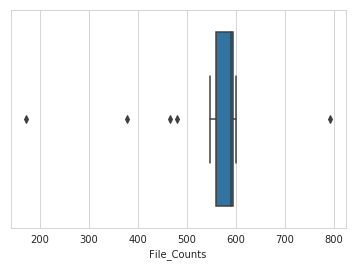
\includegraphics[width=0.48\textwidth]{figs/figure1_box_plot.png}
  \end{center}
  \caption{Box plot of the file counts per category in the training data.}
  \label{fig:box-plot-counts}
\end{wrapfigure}

\begin{figure}[t]
 \begin{center}
	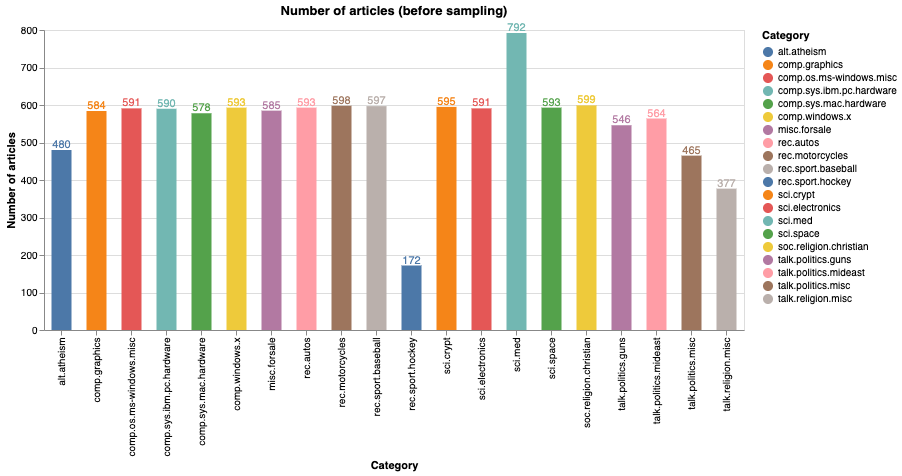
\includegraphics[width=18cm]{figs/figure1_bf_sampling.png} \\
	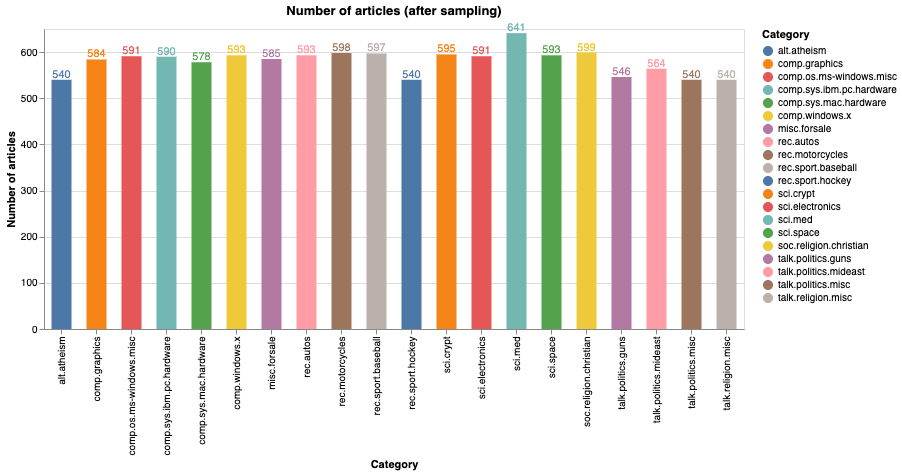
\includegraphics[width=18cm]{figs/figure1_after_sampling.png}
  \end{center}
  \caption{Comparison the sample size per class before and after sampling in the training data.}
  \label{fig:bf-vs-after-sampling}
 \end{figure}

Another concern is the length of the document: different length is correspond to different word frequency and thus may affect our TF-IDF score (Section \ref{sec:data-reprep}) and cause result biased.
There are some exceedingly long documents in the raw data (Figure \ref{fig:bf-vs-after-truncation} top pannel), so we remove the documents that has length longer than the 95th percentile, and we can see that the length distribution across categories is similar after truncation (Figure \ref{fig:bf-vs-after-truncation} bottom pannel). 

\begin{figure}[t]
 \begin{center}
	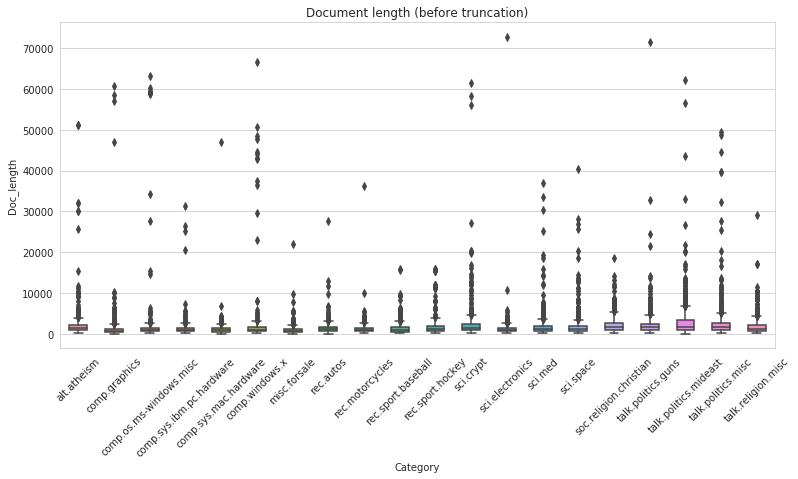
\includegraphics[width=14cm]{figs/fig3_length_bf_truncation.png} \\
	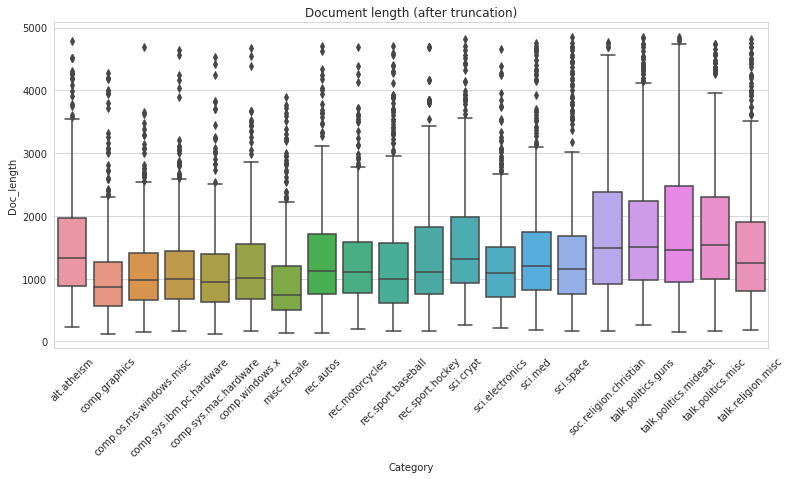
\includegraphics[width=14cm]{figs/fig3_length_after_truncation.png}
  \end{center}
  \caption{Comparison the document length per class before and after truncation in the training data.}
  \label{fig:bf-vs-after-truncation}
 \end{figure}
 
\paragraph{Code reference.}
Please refer to {\em /text-document-classifier/02. Exploratory Data Analysis} for details.

%%% 
\subsection{Feature Engineering} \label{sec:fea-eng}
In this section, we will discuss how to clean, normalize and represent the data.  The procedure in this section is performed over both training and testing data set.

\subsubsection{Data Cleaning}

The raw data consists of some redundant characters that have no prediction power, so we will remove them. Before removing these characters, we convert the documents to lower cases, assuming upper and lower cases have the same meaning.
Then we remove following redundant characters:
\begin{enumerate}
	\item Special characters while reading the text document, such as \texttt{$\backslash$n}
	\item Punctuation signs such as \texttt{.,:"/@\%}
	\item Numbers
	\item Stop words serving as connection words such as \texttt{too, from, its}
	\item Possessive pronounce and other words that are common documents but no prediction power in this data set,  such as \texttt{subject, re, et al}
\end{enumerate}

After cleaning, the content in the document is a document of meaningful words that can be used to predict the category.

\subsubsection{Data Normalization: Stemming and Lemmatization}

Since one word can have different forms, we can recover the base form by lemmatization or generate new words using stemming. Stemming is a more aggressive method in model prediction (as it generate new words). We have more than 10,000 documents and thus we can reply on {\em lemmatization only} to modify words in the data set. 

\subsubsection{Data Representation}
\label{sec:data-reprep}
For the response variable, we convert the category to numerical numbers by mapping them to $\{0, 1, \ldots, 19\}$. For the simplicity, we won't list the exact mapping in the report.
For the predictors, there are several methods to create features from text:
\begin{enumerate}
	\item Word Count Vector. We can count the frequency of each words in the document, where words are from the corpus. 
	\item TF-IDF Vector. It is short for {\bf T}erm {\bf F}requency - {\bf I}nverse {\bf D}ocument {\bf F}requency.  to present the relative importance of the words in this document and the entire corpus. 
	\item Word Embeddings. The position of the word is learned from the text based the word itself and the words around it. 
\end{enumerate}

There are other methods, and we won't list them here. In this project, we used TF-IDF for our feature engineering because it is a simple but fast and effective strategy to yield good results in text document classification. 
The idea of TF-IDF  is based on word frequency to convert text to vectors, without taking account the order or the sequence of the words.  Let $TF_i(x)$ be the frequency of word $x$ in a document $i$, and $N(x)$ be the total count in the data set.  We can calculate the inverse document frequency, $TDF(x) = \log\left(\frac {N + 1} {N(x) + 1}\right) + 1$. Then the TF-IDF score is defined as $TF(x) \times IDF(x)$, which calculates the importance of a word in one document relative to the corpus. We can use the complete word set as the corpus in this project.

We can also tune parameters in this process, including the number of grams (i.e., the number of tokens), maximum and minimum document frequency (DF) and maximum feature numbers. The following table showes the parameters in this project:
\begin{center}
\begin{tabular}{ |c|c|c|c| } 
 \hline
n-gram range & max DF & min DF & max features \\
\hline
\{1, 2\} & 100\%  & 10\% & 500 \\
 \hline
\end{tabular}
\end{center}

It is possible to further tune these parameters, but due to time constraint, I used these parameters for simplicity. 

\paragraph{Code reference.}
Please refer to {\em /text-document-classifier/03. Feature Engineering} for the details of data cleaning, normalization and representation.

%%
\subsection{Predictive Model}
After constructing our features, we can train predictive models using the training data. Taking both time and data size into consideration, I choose classical machine learning methods rather than deep learning models. Let me explain the models that I used briefly.

\paragraph{Random Forest.} 
It is a bagging method that aggregates the results from multiple decision trees using re-sampled features. Random forest in general can generate moderately good results for categorical data. 
% \paragraph{Support vector machine.}  
% It is a common classification method that aims to maximize the margin between each categories, in which we need to specify the kernel for non-linear relationship in the data. However, we have 20 categories, I don't expect it to generate a very good testing result. 
\paragraph{Multinomial Logit Model.} 
It is in the generalized linear model family, and used (multinomial) logit function as a link function. Since we have 500 features, linear combination of predictors should be enough to predict the category.
\paragraph{Naive Bayes Model.}
It assumes independency between features and applies the Bayes rule to maximize the marginal probability. Since this assumption is usually assumed to be true in text document, it is a useful method in document classification. Another big advantage is that it runs pretty fast compared with other complex methods. 
\paragraph{K-nearest Neighbor Model.}
It is non-parametric model by taking account the K-nearest neighbors. We have more than 10,000 data in the training set, it will take time to compute the distances. 

Most of these models (except naive Bayes) need to tune hyper parameters, and we applied two rounds of cross validation to choose tuning parameters. The first round is a random search, which can search over a large range of parameters (along with cross validation). Then we zoom in the neighbors of the selected parameters and perform a more fine-grid search (along with cross validation). The scoring metric is ``accuracy"/ ``f1\_weighted"  in the model training. I didn't have time to re-run the code to unify the score metric, but the difference should be mild.

\paragraph{Code reference.}
Please refer to {\em /text-document-classifier/04. Model Training} if you are interested in the tuning parameters for each method used in this project.

\section{Numerical Results}

Given a result for an estimate, it can be either true positive (TP), false positive (FP), true negative (TN) or false negative (FN). 
There are several metrics to measure the performance: accuracy, precision, recall, F1 score, area under the ROC curve and other. Among all, precision measures the ``accuracy" of our selected set, defined as TP $/$ (TP + FP) and recall measures the percentage that we pick the true ones, defined as TP $/$ (TP + FN).  In this project, we are required to use the F1 score, which is harmonic mean of precision and recall. 
We have F1 score for each category, defined as [2 precision * recall / (precision + recall)], and then we calculated the final F1 score weighted by the size of each category for comparison. I also added the accuracy as a reference, which is defined as (TP + TN) / (TP + TN + FP + FN).
(I didn't store the training F1 score, so it is missing from the table.)

\begin{center}
\begin{tabular}{ |c|c|c|c| } 
 \hline
\multirow{2}{*}{Model} & \multicolumn{1}{c|}{F1 Score}  & \multicolumn{2}{c|}{Accuracy}  \\
\cline{2-4}
 & Testing & Training & Testing \\
 \hline
 Multi-logit & 63\% & 81\% & 63\% \\
 Naive Bayes & 62\% & 74\% & 62\% \\
 Random Forest & 59\% & 100\% & 59\%\\
 KNN & 54\% & 100\% & 54\%\\
 \hline
\end{tabular}
\end{center}

From the table, the F1 score and accuracy are consistent and the multinomial logistic (multi-logit) achived the best testing F1 score and accuracy. Random forest and KNN were overfitting the data, and thus the testing results were not desirable. Naive Bayes had comparable performance with multi-logit, and it was taking much less time. 
We can take a closer look at the confusion matrix of the multinomial logistic model  using testing data (Figure~\ref{fig:conf-mat}), where the large values in the diagonal show its good performance.

\begin{figure}[t]
 \begin{center}
	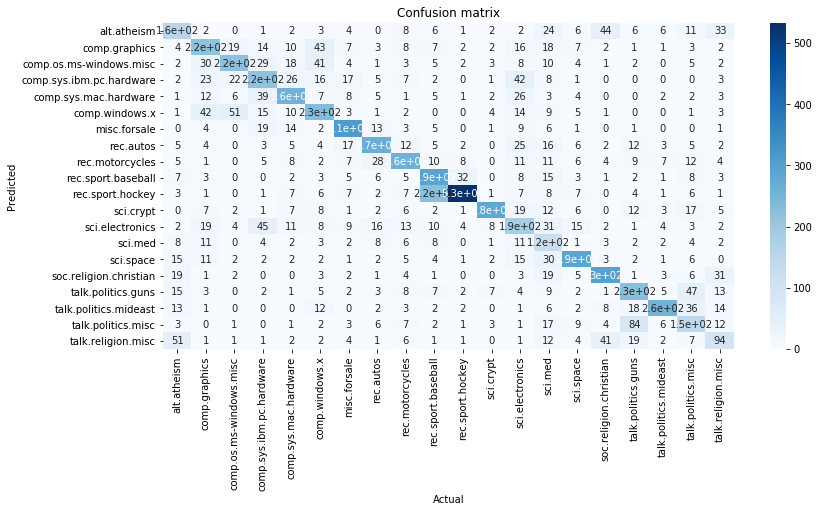
\includegraphics[width=15cm]{figs/fig4-confusion-matrix.png}
 \end{center}
  \caption{Confusion matrix of the multinomial logistic model (test data).}
  \label{fig:conf-mat}
\end{figure}
 
\section{Conclusion}

In this project, we constructed a text classifier from the original documents using a simple approach, and achieved prediction accuracy and F1 score up to 63\%. %, including data generation, exploratory data analysis, data cleaning, lemmatization, data representation, model training and testing, and numerical results presentation. 
Due to the time limit, there are still possible improvements. One of those is to represent data using more strategies and thus create more features. Another one is that one can tune hyper parameters using a more finely-defined grid to generate better hyper parameter if having time budget. Last but not the least, there are other potential useful information to extract from the original document, such as email address, that I didn't take the full advantages of. Overall, it is an exciting project and the result definitely has room to improve. 

% \bibliographystyle{plainnat}
%\bibliographystyle{unsrt}
% \bibliography{./cite2}
\end{document}

